%----------------------------------------------------------------------------------------
%	PACKAGES AND OTHER DOCUMENT CONFIGURATIONS
%----------------------------------------------------------------------------------------


\documentclass[12pt,oneside,final,a4paper]{report}
\usepackage{generators/imports}
\usepackage{tikz}
\addbibresource{generators/refs.bib}
%\makeglossaries      % alt 1
\makenoidxglossaries  % alt 2

\renewcommand*{\acronymname}{List of Acronyms and Abbreviations}
\renewcommand{\glsnamefont}[1]{\textbf{#1}}

%Create acronyms here.
\newacronym{ide}{IDE}{Integrated Development Environment}
\newacronym{fsa}{FSA}{File System Abstraction}
\newacronym{asr}{ASR}{Abstract Semantic Representation}
\newacronym{ast}{AST}{Abstract Syntax Tree}
\newacronym{stf}{STF}{Syntactic Theory Functor}
\newacronym{saas}{SaaS}{Software as a Service}
\newacronym{vcs}{VCS}{Version Control System}
\newacronym{html}{HTML}{HyperText Markup Language}
\newacronym{mvc}{MVC}{Model-View-Controller}
\newacronym{ui}{UI}{User Interface}
\newacronym{json}{JSON}{JavaScript Object Notation}
\newacronym{gui}{GUI}{Graphical User Interface}
\newacronym{dom}{DOM}{Document Object Model}
\newacronym{vdom}{VDOM}{Virtual Document Object Model}
\newacronym{rsms}{RSMS}{Rust Module System}
\newacronym{jsms}{JSMS}{JavaScript Module System}
\newacronym{lsp}{LSP}{Language \gls*{ls}}
\newacronym{ls}{LS}{Language Server}
\newacronym{npm}{NPM}{Node Package Manager}
\newacronym{moa}{MoA}{Mathematics of Arrays}
\newacronym{bldl}{BLDL}{Bergen Language Design Laboratory}
\newacronym{vim}{Vim}{Vi Improved}
\newacronym{api}{API}{Application Programming Interface}
\newacronym{mdcs}{MCDS}{Multi-way Dataflow Constraint System}
\newacronym{abi}{ABI}{Application Binary Interface}
\newacronym{e2e}{E2E}{End-To-End}
\newacronym{dag}{DAG}{Directed Acyclic Graphs}
\newacronym{css}{CSS}{Cascading Style Sheets}
\newacronym{ipc}{IPC}{Inter-Process Communication}
\newacronym{dsl}{DSL}{Domain Specific Language}
\newacronym{vscode}{VS Code}{Visual Studio Code}
\newacronym{rest}{REST}{Representational State Transfer}
\newacronym{mpsc}{MPSC}{Multi Provider Single Consumer}
\newacronym{smt}{SMT}{Satisfiability Modulo Theories}
\newacronym{os}{OS}{Operative System}
\newacronym{io}{IO}{Input/Output}
\newacronym{cpu}{CPU}{Central Processing Unit}
\newacronym{ub}{UB}{Undefined Behavior}
\newacronym{cli}{CLI}{Commandline Interface}
\newacronym{cicd}{CI/CD}{Continuous Integration and Continuous Delivery}
\newacronym{erpc}{Eclipse RPC}{Eclipse Rich Client Platform}

\newglossaryentry{git}
  { name={Git}
  , description={Git is a \gls*{vcs} for tracking changes in computer files and coordinating work on those files among multiple people}
  }
\newglossaryentry{intellij}
  { name={IntelliJ}
  , description={IntelliJ is an \gls*{ide} for Java}
  }
\newglossaryentry{eclipse}
  { name={Eclipse}
  , description={Eclipse is an \gls*{ide} for Java}
  }
\newglossaryentry{nvim}
  { name={Neovim}
  , description={Fork of \gls*{vim}}
  }

\begin{document}
%----------------------------------------------------------------------------------------
%	TITLE PAGE
%----------------------------------------------------------------------------------------

\begin{titlepage} % Create the command for including the title page in the document
  \fontfamily{phv}\selectfont
  \centering % Center all text

  %----------------------------------------------------------------------------------------
  %	TITLE SECTION
  %----------------------------------------------------------------------------------------

  \vspace{200pt}
  {\Huge Developing a zero-core modular IDE} \\ % Title
  \vspace{5pt}

  {\Large \textsl{Creating a zero-cost IDE; you get what you pay for}} % Subtitle or further description
  \vspace{50pt}

  %----------------------------------------------------------------------------------------
  %	AUTHOR SECTION
  %----------------------------------------------------------------------------------------

  \LARGE{\textbf{Nils Michael Fitjar}}\\ % Author name

  \vfill % Whitespace between the author name and the school

  %----------------------------------------------------------------------------------------
  %	DESCRIPTION AND DATE SECTION
  %----------------------------------------------------------------------------------------


  {\Large \textbf{Master's thesis in Software Engineering at} \\
  \vspace{10pt}
  Department of Computer science, Electrical engineering and Mathematical sciences, \\
  Western Norway University of Applied Sciences \\
  \vspace{10pt}
  Department of  Informatics, \\
  University of Bergen \\}
  \vspace{10pt}
  {\large \monthyeardate\today} % Month and year published

  %----------------------------------------------------------------------------------------
  %	LOGO SECTION
  %----------------------------------------------------------------------------------------

  \vfill % Whitespace between the school and the publisher logo


  \begin{figure}[h!]
    \captionsetup[subfigure]{labelformat=empty}
    \subfloat[][]{\includegraphics[height=70pt]{logos/hvl_logo_engelsk.pdf}}
    \hfill
    \subfloat[][]{\includegraphics[height=70pt]{logos/uib-logo.eps}}
  \end{figure}


\end{titlepage}

\pagenumbering{roman}

\begin{abstract}

  This paper introduces a Modular, \textit{Zero Core}, Application, to serve as
  an Integrated Development Environment (IDE) for experimental programming
  languages, addressing limitations in traditional IDEs. While standard IDEs are
  crucial in software development, their support for experimental languages is
  often inadequate. This can and, has been solved by extensively using the
  plugin/module architecture of existing IDEs. However, relying on
  \textit{niche} plugins/functionality is not future safe.
  % TODO: Rewrite this sentence
  This project proposes a modular IDE to extend its lifespan and enhance support
  for experimental languages. Analyzing the essential features of traditional
  IDEs and the need for adaptability to new paradigms and tools. Magnolia, a
  research programming language developed at UIB, serves as a case study,
  highlighting its unique characteristics and the necessity for a specialized
  IDE. The primary research question explores how modularization facilitates the
  design and implementation of experimental programming languages. Specific
  modules tailored for experimental languages, including Abstract Semantic
  Representation (ASR) Transformation, Term Algebras, MoA translation, and
  Syntactic Theory Functor (STF), are outlined. To showcase the usefulness of
  a modular approach, the modules needed to extend the core application to an
  IDE will be implemented.
  %\keywords{Modularization \and IDE \and Magnolia.}

\end{abstract}

\renewcommand{\abstractname}{Acknowledgements}
\begin{abstract}
	Est suavitate gubergren referrentur an, ex mea dolor eloquentiam, novum ludus suscipit in nec. Ea mea essent prompta constituam, has ut novum prodesset vulputate. Ad noster electram pri, nec sint accusamus dissentias at. Est ad laoreet fierent invidunt, ut per assueverit conclusionemque. An electram efficiendi mea.

	\vspace{1cm}
	\hspace*{\fill}\texttt{Nils Michael Fitjar}\\
	\hspace*{\fill}\today
\end{abstract}
\setcounter{page}{1}
\newpage

\include{generators/tableOfContentsAndListings}
\pagenumbering{arabic}
\setcounter{page}{1}
\setlength{\parskip}{0.5cm plus4mm minus3mm}

\chapter{Introduction}

Standard \gls{ide}s are indispensable tools in software development, offering features
like early bug reporting, project outline visualization, code highlighting, and
code completion However, these \gls{ide}s may not adequately support the unique
demands of experimental programming languages.
% Rewrite this
To solve this, a modular approach is used to designed and \gls{ide}.

\section{Experimental Languages}

Talk about Abstract Semantic Representation (ASR) Transformation,
Term Algebras, Mathematics of Arrays, and Syntactic Theory Functor (STF)

\section{Integrated Development Environment}

\todo{Rewrite this}
An \gls{ide}, aids a developer, as all the
needed tools for development are integrated into one application. There are
different kinds of \gls{ide}, generic and specialized.

A specialized \gls{ide} is one targeted towards a specific language, like Eclipse,
(reference?), or IntelliJ (reference?), which target Java/JVM. It contains
specialized features like:

\begin{itemize}
  \item Syntax Highlighting
  \item Code Autocompletion
  \item Go-to-definitions
  \item \dots
\end{itemize}

A lot of these features are possible due to \textit{Language Server Protocols},
which allow for a standardized way for compilers to give code-support to \gls{ide}'s.

\todo{Connect these better}

A generic \gls{ide} contains the features that are common among development in any
programming language, like:

\todo{Should write a paragraph or two about each of these points}
\begin{itemize}
  \item File explorer
  \item Project manager
  \item Version Control System integration
\end{itemize}


\chapter{Background}

\section{Magnolia}

Magnolia is an experimental research language being developed \gls{bldl} at the
University of Bergen. Magnolia is designed to support a high level of abstraction
and ease of reasoning. This is achieved by \textit{concepts}, \textit{axioms} and
\textit{implementations}.

\todo{
  Add some reason for this way of thinking, with an example of real usage of
  semigroups, like some kind of API
}

Sets with specific operations acting on those elements, known as algebraic
structures, showcase the usage of concepts. Magma consists of a set with just a
singular binary operation, that must be closed by definition. A semigroup is an
extension of magma, with the added property that the binary operation is
associative. A monoid is an extension of a semigroup, with the added property
wherein an element in the set, \textit{C}, sometimes called a \textit{unit}, or
the \textit{identity}. This \textit{identity} ensures the following equation
holds, where the binary operation is $ \oplus $, and $ a, C $ are elements of the set.

\begin{equation}
  a \oplus C = a
\end{equation}

This, again, can be extended with an additional property, namely,
\textit{inverse element}.

\begin{equation}
  \forall a, \exists b, \in M \implies a \oplus b = C
\end{equation}

Assuming associativity.

This structure could be implemented in something like Java, an Object-Oriented
Language, as shown in listings \ref{lst:jmagma}, \ref{lst:jsemigroup},
\ref{lst:jmonoid}, and \ref{lst:jgroup}. Note the empty interfaces; there is
nothing that enforces the different laws on the properties. This can only be
done by unit testing, which is not enforced on a consumer of the \gls{api}.

\begin{center}
  \lstinputlisting
    [ language=Java
    , caption={Magma concept in Java}
    , label=lst:jmagma]{./code/magma.java}
\end{center}

\begin{center}
  \lstinputlisting
    [ language=Java
    , caption={Semigroup concept in Java, can only be upheld using unit tests}
    , label=lst:jsemigroup]{./code/semigroup.java}
\end{center}

\begin{center}
  \lstinputlisting
    [ language=Java
    , caption={Monoid concept in Java, can only be upheld using unit tests}
    , label=lst:jmonoid]{./code/monoid.java}
\end{center}

\begin{center}
  \lstinputlisting
    [ language=Java
    , caption={Group concept in Java, can only be upheld using unit tests}
    , label=lst:jgroup]{./code/group.java}
\end{center}

In Magnolia, however, this can be enforced on the \textit{interface}-level. The
example code shown in listing \ref{lst:magma}, showcases a concept
representation a binary operation, which has one function, \textit{magma}, which
takes in two values of type \textit{T}, and returns \textit{T}. Note that the
actual implementation of this function is missing. This is because a concept
encodes the properties of a users code. The actual implementation of the
\textit{magma} function needs to uphold the properties of the concept that is
being implemented. In this case, it is just that the input and output
of the function are of the same types.

\begin{center}
  \lstinputlisting
    [ language=Magnolia
    , caption={Magma concept in Magnolia}
    , label=lst:magma]{./code/magma.mg}
\end{center}

In the example code shown in listing \ref{lst:semigroup}, the \textit{magma}
concept has been expanded upon, still following the same rules as before, but
with the added property of associativity.

\begin{center}
  \lstinputlisting
    [ language=Magnolia
    , caption={Semigroup concept in Magnolia}
    , label=lst:semigroup]{./code/semigroup.mg}
\end{center}

\begin{center}
  \lstinputlisting
    [ language=Magnolia
    , caption={Monoid concept in Magnolia}
    , label=lst:monoid]{./code/monoid.mg}
\end{center}

\begin{center}
  \lstinputlisting
    [ language=Magnolia
    , caption={Group concept in Magnolia}
    , label=lst:group]{./code/group.mg}
\end{center}

\section{Reusable Software}

\subsection{Reuse in Magnolia}

\subsection{Software Lifetimes}

Software in general, lasts around 30 years (source). This is quite a long time,
but, this statistic is about more \textit{rigid} applications, which have an
unchanging scope. In more \textit{chaotic} fields, this number is reduced, as
paradigm shifts within certain fields, which results in the need for drastic
changes in the existing applications, where the needed work to change the code,
can be more than to create a new application.

\subsection{Software Longevity}

Most examples of \textit{popular} software, are open source, like \gls{vim}.
\gls{vim} is a text editor which has been in use since 1991. There are several
factors behind this success, but the ones being highlighted here, are due to its
extensibility and due to it being open-sourced. Being open sourced, allows for a
rotating cast of maintainers, ensuring the core application has the features its
users wants. The users of \gls{vim} can be split into two categories,
\textit{standard users}, and \textit{plugin developers}. \gls{vim} has an
extensive plugin ecosystem, which can extend \gls{vim}s functionality from a
text editor, to a fully fledged \gls{ide}.

\section{Integrated Development Environment}

An \gls{ide}, aids a developer, as all the needed tools for development are
integrated into one application. There are two different kinds of \gls{ide}s,
generic and specialized. \todo{Source}

A specialized \gls{ide} is one targeted towards a specific language, like
Eclipse, (reference?), or IntelliJ (reference?), which target Java/JVM. It
contains specialized features like the following:

\paragraph{Syntax Highlighting} Highlighting important keywords, identifiers
and more, makes the language easier to read for the developer, allowing them to
spot easy to miss errors, like misspelling of keywords.

\paragraph{Code Autocompletion} Suggesting keywords, method names or even entire
code snippets, is a powerful tool an \gls{ide} can have. This is possible to
achieve, in some form, without being specialized, by for example, suggesting
text that already exist in the document, but is most useful if it is
specialized, and can suggest built-in methods. This allows a developer to not
having to remember exactly how methods are named, is the method to split a
string by some delimiter, \textit{split\_by} or \textit{split\_on}? As long as
the developer writes \textit{split}, the correct method name will be suggested.

\paragraph{Go-To-Definitions} Being able to quickly navigate to methods and read
their implementation is a useful tool for a developer, as less time has to be
spent navigating the project structure, to figure out where some method was
implemented, and more time can be spent actually developing.

A lot of these features are possible due to \textit{Language Server Protocols},
which allow for a standardized way for compilers to give code-support to
\gls{ide}'s.

A generic \gls{ide} contains the features that are common among development in
any programming language, like:

\paragraph{File Explorer} Most project nowadays is larger than one file, so
being able to visualize the project in a tree-like-structure, and navigate that,
is useful. This feature usually comes with the ability to manipulate the project
structure, by adding files, folders, moving files around, and deleting them.

But creating any \gls{ide} would still limit the lifetime of the application.
The best example of a long living active \gls{ide}, or, at least editor, is Vim
(source?). Vim is not a feature full editor, but it is simple, lightweight, and
works on any operating system. But most people use it, for how easy it is to
extend; Its lifetime has been greatly extended by the ease of modularization.
Any popular module for Vim is open-source, and therefore, if any module had an
active community around it, if the \textit{lead} developer of the module stopped
developing it, that community can continue to develop the module, either by
getting maintenance access to the repository, or by forking it. Ensuring the
lifetime of the module is extended.

\subsection{Module Architecture}

\todo{Talk about modules in IDEs}

\todo{Find a way to mention this?}
\paragraph{Language Agnostic} The largest limiting factor in module oriented
applications, is the \textit{language barrier} Most applications limit what
language one can extend an application with, like in "Visual Studio Code", where
its JavaScript/HTML/CSS. Or IntelliJ, where one can use Java or Kotlin. But what
does language agnostic mean in the context of programming languages? It is, and
always will be C. Any \textit{serious} language can create some bindings with C.
So, for a module application to be Language Agnostic, it must be able to use C
Modules. This just means that the application must be able to call function from
a C library.

\subsection{Language Workbench}
\todo{Expand}
I don't know what this is.

\subsection{Language Server}

The most important features in a modern \gls{ide} are possible due to the
\gls{lsp}. \gls{lsp} is a protocol for a language server and editor,
(the client), with which they communicate, allowing for features like code
completion, syntax highlighting, marking of warnings and errors, as well as
refactoring routines. This client-server architecture, in \gls{ide}s are a
more recent development (2020s), as previously, support for the features
mentioned, were only possible due to specific modules being written for
specific \gls{ide}s. \gls{lsp} being the norm, is a sign of modularity being
preferred, as now a single \gls{lsp} can be created, and used across several
different applications, like IntelliJ, VS Code and Vim. While useful for
\textit{standard} language, this is the limiting factor when it comes to
supporting experimental languages, as not only does a new set of protocols need
to be appended to a language server, the editor itself needs to be changed to
actually use these protocols. This creates a lot of work, for both the \gls{ide}
developer and for the compiler developer. Here is where a modular approach can
help both. If some new functionality or feature is added to the experimental
language, this off course means the compiler/interpreter has to be expanded
and/or modified, but for the \gls{ide}, a module could be added/modified to
utilize this change, instead of having to change the entire application.

In this paper, we will start by discussing some background around modularity,
software longevity, and Magnolia (chapter 2). We will also discuss the different
ways to achieve modularity within an application, and point out different
behaviors that arise from such a setup (chapter 4). Finally, we will discuss the
results (chapter 5), and conclusions (chapter 6).

Traditional \gls{ide}s encompass essential features such as syntax highlighting, code
navigation, and hover-help, playing a crucial role in the software development
process. However, their limitations become apparent when working with
experimental languages. This paper advocates for modularization and
\textit{composability} as key design principles, demonstrating their ability to
extend the operational lifespan of software by allowing for ease-of adoption to
new paradigms and tools. The discussion revolves around Magnolia, an
experimental research programming language developed by \gls{bldl} at the
University of Bergen. Magnolia will act as a case study illustrating the need for
a specialized \gls{ide}. It is a way to experiment with novel language features.
And to achieve this in a sufficient manner, a more specialized \gls{ide} is
required.


\section{Existing Magnolia IDE}

The current \gls{ide} for Magnolia, is a many-years-old version of Eclipse,
using modules and functionality from the core Eclipse application, that has
since been outdated. The \gls{ide}s lifetime was limited by a dependency on
external modules and features that where not maintained by \gls{bldl}. This
meant that for future development of Magnolia, an outdated \gls{ide} was needed,
with outdated tooling. Furthermore, the Magnolia compiler was implemented as an
Eclipse module, which means that development is limited to Eclipse, and only
Eclipse, as a developer cannot compile Magnolia code without it.

Having the entire application available \textit{in-house}, will also help, as
open source; availability to the source code helps when developing niche
modules.

Modularization will help to mitigate some of the issues with the current
Magnolia \gls{ide}. Instead of maintaining an entire application, the needed and
wanted features of the application can be maintained instead.

Experimental languages might have features which are not possible to be fully
used in current \gls{ide}s. This is also the case for the current Magnolia
\gls{ide}. The compiler for Magnolia, syntax highlighting, error reporting, and
hover-functionality are functionality made in the Eclipse \gls{ide}, by using
its plug-in architecture. Some of the functionality and plug-ins this
implementation used, have been deprecated in later version of Eclipse. This
means the Magnolia \gls{ide} is locked to an old version of Eclipse, which, as
time passes, increases the complexity of installation, as the surrounding
tooling and libraries needed by this version of Eclipse also becomes deprecated.
Currently, in INF220, at the university, two weeks are set aside for students to
be able to install it.

\todo{Reference Anya's paper}


\chapter{Magnolia IDE} \label{cha:ide}

This section will discuss the new Magnolia \gls{ide}, the different users of the
\gls{ide}, and their possible experiences which was under consideration when
developing the application.

\section{User Perspectives}

This application has to consider different users. In \gls{ide}'s like
\gls{eclipse} or \gls{intellij}, there is the primary user base, the developers
who are using the \gls{ide} to develop, and then there are the secondary user
base, the developers whom develop \textit{plugins} for the \gls{ide}. Being the
primary user base, most of the new features implemented by either \gls{ide} are
related to the development experience. There are still changes to that the
\textit{plugin} developers are interested in, namely \gls{api} changes.
\gls{intellij} for example, lists their \textit{incompatible \gls{api} changes}
\cite{intellijBrokenApi}. Breaking changes between \gls{ide} versions is
something normal users of the \gls{ide} do not worry about. As usually when a new
version is released, it means more features for the developer to utilize. While
\textit{plugin} developers have to ensure their \textit{plugins} still work. One
of the reasons behind \gls{ide} version changes can break a \textit{plugin}, is
due to how they interact with their \gls{ide}. In \gls{intellij} a
\textit{plugin} is created by implementing a Java interface for the functionality
one wants.

If one wanted \gls{intellij} to recognize that a file with the extension "rs",
is a Rust source file, and give it a certain icon, one would have to implement
the \textbf{Language} interface and override the \textbf{getIcon} method to
return the wanted icon.

So a change in the \gls{ide} architecture could break a \textit{plugin} for the
newer version of the \gls{ide}, as with Bagge's Magnolia \gls{ide}
\cite{baggeIde}. While in this zero core \gls{ide} module developers are quite
important, as they are the ones who add the functionality to the \gls{ide}.
Therefore, the core \gls{api} has to be more stable, and it is by virtue of not
having much functionality.

\section{Module Developer}

Being a zero core application; all functionality comes from modules, the module
developer experience is the most important. To achieve this, documentation is
important. If a module developer has a question about how the core might react,
it should be answered by the documentation. In \gls{eclipse}, this is in the
form of \textit{Javadoc}s, which specify, with examples how the \gls{eclipse}
runtime handles \textit{plugins}. \footnote{\url{https://help.eclipse.org/latest/rtopic/org.eclipse.platform.doc.isv/reference/api/org/eclipse/core/runtime/Plugin.html}}

The documentation for \textit{plugin} developers, in both \gls{intellij} and
\gls{eclipse} has to be large, due to of how \textit{plugins} interact with the
\gls{ide}; it is a large \gls{api}. In a zero core \gls{ide} it is smaller,
simply due to the fact that the core \gls{ide} offers fewer features, as features
necessarily come from a module.

\subsection{Language Agnostic Modules}

The largest limiting factor in module oriented applications, is the
\textit{language barrier} Most applications limit what language one can extend
an application with, like in \gls{vscode}, where its JavaScript/HTML/CSS. Or
\gls{intellij}, where one can use Java or Kotlin. But what does language agnostic
mean in the context of programming languages? It is, and always will be C. Rust,
the language chosen to implement this \gls{ide}, also has bindings to C. This
means that Rust can invoke C libraries. This is important for language
agnosticism, as any language that has bindings to C, has then, through C,
bindings to Rust. This is called an \gls{abi}, specifically the C-\gls{abi}.

\begin{figure}
  \begin{center}
    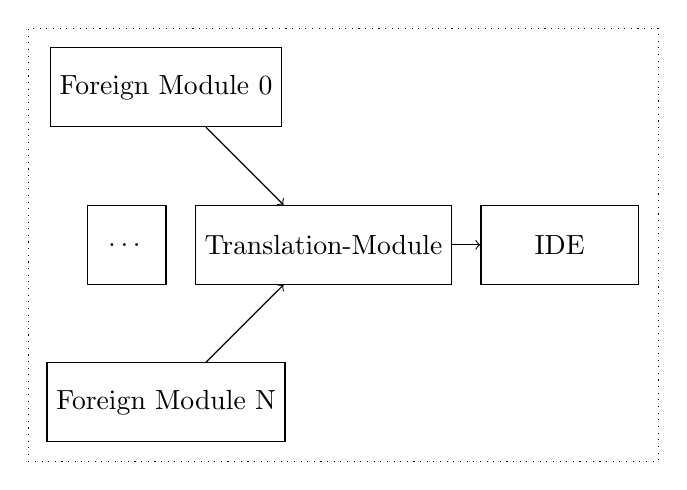
\begin{tikzpicture}
  % Nodes
  \node (b) [rectangle, draw, minimum height=5.5cm, minimum width=8cm, dotted] at (-1.75, 0) {};
  \node (p-0) [rectangle, draw, minimum height=1cm, minimum width=2cm] at (-4, 2) {Foreign Module 0};
  \node (dots) [rectangle, draw, minimum height=1cm, minimum width=1cm] at (-4.5, 0) {\dots};
  \node (p-n) [rectangle, draw, minimum height=1cm, minimum width=2cm] at (-4, -2) {Foreign Module N};
  \node (m) [rectangle, draw, minimum height=1cm, minimum width=2cm] at (-2, 0) {Translation-Module};
  \node (i) [rectangle, draw, minimum height=1cm, minimum width=2cm] at (1, 0) {IDE};
  % Arrow
  \draw[->] (m) -- (i);
  \draw[->] (p-0) -- (m);
  \draw[->] (p-n) -- (m);
  % Header
\end{tikzpicture}

    \caption{Foreign modules being invoked by a singular Translation-module}
    \label{fig:fm1}
  \end{center}
\end{figure}

\begin{figure}
  \begin{center}
    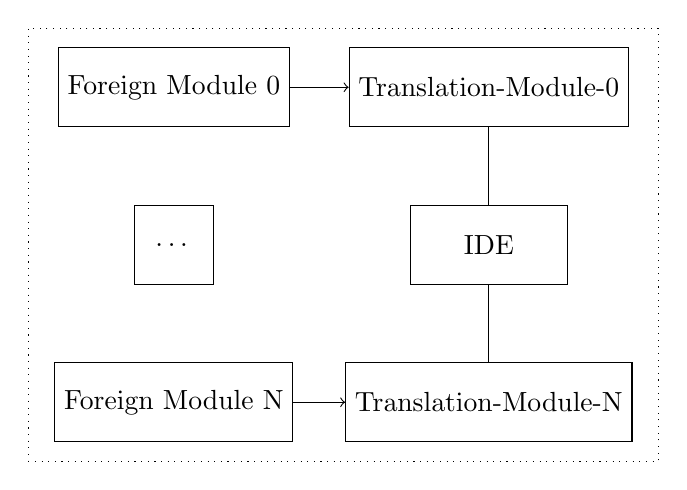
\begin{tikzpicture}
  % Nodes
  \node (b) [rectangle, draw, minimum height=5.5cm, minimum width=8cm, dotted] at (-2.85, 0) {};
  \node (p-0) [rectangle, draw, minimum height=1cm, minimum width=2cm] at (-5, 2) {Foreign Module 0};
  \node (dots) [rectangle, draw, minimum height=1cm, minimum width=1cm] at (-5, 0) {\dots};
  \node (p-n) [rectangle, draw, minimum height=1cm, minimum width=2cm] at (-5, -2) {Foreign Module N};
  \node (m-1) [rectangle, draw, minimum height=1cm, minimum width=2cm] at (-1, 2) {Translation-Module-0};
  \node (m-n) [rectangle, draw, minimum height=1cm, minimum width=2cm] at (-1, -2) {Translation-Module-N};
  \node (i) [rectangle, draw, minimum height=1cm, minimum width=2cm] at (-1, 0) {IDE};
  % Arrow
  \draw (m-1.south) -- (i);

  \draw (m-n.north) -- (i);

  \draw[->] (p-0) -- (m-1);
  \draw[->] (p-n) -- (m-n);
\end{tikzpicture}

    \caption{Foreign modules being invoked by an individual Translation-module}
    \label{fig:fm2}
  \end{center}
\end{figure}

This module could be a singular one, acting as a translator, translating the
data flowing between the core and foreign-modules as shown in figure
\ref{fig:fm1}, or each foreign-module could have their own translator as shown
in figure \ref{fig:fm2}. For some languages such a setup would be necessary.
A Haskell module, for example, would require some translation module, either a
unique translator for each module, where the Rust module would start the
required Haskell runtime \cite{ghcRts}, when invoking the Haskell module, and
exit before returning, avoiding \gls{ub}. The reason Haskell is of interest,
is that the new compiler is written in Haskell \cite{wiig}, and as such, if one
where to develop \gls{lsp} capable modules for the \gls{ide}, a translation
module from Rust to Haskell is necessary.


But this language agnosticism also means that
translating from one language to another should be trivial. This is achieved by
the models used in the core. The \textit{primitive} types, are the same as in
JavaScript, the notion of an empty value, numbers, strings, lists and
\textit{objects}, can be serialized/deserialized to/from any language. So the
manipulation on these types can be extracted and rewritten in another preferred
language. Therefore, to be fully language agnostic, modules should be
syntactically translatable between each other. The same two modules, one
implemented in JavaScript, the other in Rust, should be semantically the same.

\subsection{Existing Third Party Libraries}

Since the core can support different languages, one can use the libraries
written for these languages to make an \gls{ide}. This could be achieved by
creating a module, acting as a wrapper around the library. For example, by
using JavaScript and since the core application is designed to be an \gls{ide},
one could use existing JavaScript libraries, like \textit{Monaco}, which is the
text editor used by Visual Studio Code. It comes with an integrated
\gls{lsp}-client, which would enable the application to easily support existing
popular languages.

However, being zero core, this application could be anything, from an audio
editing program, to a game emulator. Simply using the \textit{JS-DOS} library,
would allow the application to run video games like Doom.

\subsection{Module Development Experience}

A module developer can invoke the module-developer-\gls{cli}-tool to create
boilerplate modules for JavaScript, TypeScript or Rust. After they have
implemented a module, they can test it out, again by invoking the
\gls{cli}-tool. When they are satisfied with their implementation, they can add
it to the compile time configuration for the \gls{ide}, and compile it. They
can now use the module in the \gls{ide}.

\section{IDE Users}

As mentioned in chapter \ref{cha:background}, modern \gls{ide}s come with an
integrated module architecture. Which is used to extend/change the \gls{ide},
from as simple as to change the theme, to more drastic changes, like changing
all key binds to \textit{vim-motions}. In any case, a user expects certain
functionality to already exist in an \gls{ide}, like text editing. A maintainer
of a zero core \gls{ide} could supply modules added at compile time, meaning the
expected functionality is there out of the box, while more thematic modules
could be supplied as runtime modules.


\subsection{Developer}

Most users just want an \gls{ide}, and do not spend, nor want to spend, much
time configuring their \gls{ide}. This can be achieved by adding the necessary
modules to qualify as an \gls{ide} at compile time. If one is a lecturer,
teaching something that is used by a \textit{niche} programming language, the
lecturer can add the needed modules to a configuration file,
\textit{Modules.toml}, and then compile it to an \gls{ide}. Before the \gls{ide}
is compiled, it finds the mentioned modules in the configuration file, and
directly integrates them into the core, ensuring that the resulting binary is a
fully fledged \gls{ide}. And then this \gls{ide} can be distributed to the
students, who can still extend the \gls{ide} with runtime modules at their own
digression.

\section{Maintainer}

To make the maintainer of the core application most comfortable, good
documentation is needed. The same documentation a module developer wants, so
it's important for them and the maintainer that the documentation is up-to-date.
But how good is documentation if it is not updated when the code being
documented is changed? This is where Rust's doc-test system comes into play. Any
function annotated with a doc string, can contain code examples. If these code
examples are written as Rust code, and use assert statements, then this code is
run, during testing, as if it was an actual test. Meaning the saying
\textit{code is documentation}, is \textit{documentation is code} in Rust.



\chapter{Implementation} \label{cha:impl}

This section will focus on the implementation of the zero core \gls{ide}. In
section \ref{sec:stack}, we will mention technologies used, and why they were
chosen. In section \ref{sec:mod1} and \ref{sec:mod2}, we will discuss the
different iterations the application architecture had, and why they were subpar,
compared to section \ref{sec:mod3}, which is the implementation of the zero core
\gls{ide}. Section \ref{sec:testing} will explain the necessity of testing when
using such a modular design, and explore the ease of which functionality can be
tested.

\section{Tech Stack} \label{sec:stack}

A module can extend an application at either compile time, or during runtime.
This could be achieved by using an interpreted language like JavaScript or
Python. The issue with using a dynamically typed language like Python or
JavaScript, is that it enhances the risk for runtime issues occurring, and when
dealing with scenarios like writing to files, or running long processes like
compiling a program, it is important to avoid such issues. So using a typesafe
language, that can \textit{transform} runtime errors into compile time errors,
is preferred. Furthermore, being able to support runtime modules, in a language
agnostic manner, necessarily means that the core \gls{ide} needs good
\gls{abi} support, and therefore should be implemented in a low level language.
But what does \textit{low level} language mean? And what is an \gls{abi}?

\subsection{Low level languages}

Programming languages has changed over time. In the beginning, a program was a
series of ones and zeros, representing instructions a computer should do. Since
then, we have moved several abstraction layers above what is commonly referred
as \textit{bare metal} programming. From writing in hexadecimal instead of
binary, to machine instructions, to more generic programming language, like C.
What was different with C, compared to writing direct machine instructions, was
that an external program, a compiler, could translate C code to machine
instructions specific to the computers' \gls{cpu} architecture, this meant a
single program, written in C, could be compiled to many different computers. So,
at the time C came out, it was considered a \textit{high level} programming
language, because the language a developer was writing in, had a higher level of
abstraction. Today this notion of \textit{low} and \textit{high} level languages
has changed. A \textit{low level} language is close to how a \gls{cpu}
\textit{thinks}, which has traditionally meant that C is a low level programming
language, but some authors \cite{cNotLowLevel} argue that this is no longer the
case. In any case, we will use \textit{low level} to mean a programming
languages like C, where direct memory manipulations is a feature of the
language.

\subsection{Application Binary Interface (ABI)}

An \gls{abi} is an interface between two programs. This could be a
dynamic library used by a C program, where both binaries agree on how the data
is stored. The reason they need to agree on how data is ordered in the memory,
is that accessing into unowned memory could lead to \textit{undefined} behavior.

\paragraph{Undefined behavior} In programming, undefined behavior is behavior
that is not defined by the specification of the language being used.
\todo{Is this a correct explanation?}

\todo{Connect these two sections better}

\paragraph{Why not C?} C has good parts, like the C-\gls{abi}, which most
languages have bindings too. Using C would mean allowing those languages to
interface with our project, meaning, one step closer to a language agnostic
module architecture. But C has issues, like being the number one cause in
security issues. (This is just because so much of our infrastructure is written
in C, but y'know.) These security issues are mostly caused by memory management.
Would be cool if the C compiler could notify a developer if they were developing
something that could cause an issue in the future. Enter, Rust.
\todo{Rewrite this paragraph}

\subsection{Rust}

Rust is a general purpose programming language, designed for, amongst other
things, type safety, memory safety, and concurrency. When programming in Rust,
the bugs common in other languages, like null pointers, buffer overflow and data
races are detected at compile time. Most of these are features of Rusts
ownership rules. These rules, enforced by the compiler, ensure that values are
safely dropped, (freed), this ensures that all variables referenced in Rust have
a value, and can be safely evaluated. It works by simply dropping values when
they are out of scope. The example in listing \ref{lst:ownership}, the
\textbf{name} variable is declared, and used as an argument in the
\textbf{greeting} function. We cannot call the function again with
\textbf{name}, since at the end of \textbf{greeting}, before it returns,
\textbf{name} is dropped, since once we called \textbf{greeting}, the
\textbf{main} method no longer \textit{owned} \textbf{name}, as the ownership
was transferred to \textbf{greeting}. We could \textit{fix} this by changing the
argument type from \textit{name: String}, to \textit{name: \&String}, (commonly
written as \textit{name: \&str}), and adding the borrow symbol to the argument in
the method invocation, as shown in listing \ref{lst:ownership-ref}.

\begin{center}
  \lstinputlisting
    [ language=Rust
    , caption={Ownership example (Rust)}
    , label=lst:ownership
    ]{./code/rust-ownership.rs}
\end{center}

\begin{center}
  \lstinputlisting
    [ language=Rust
    , caption={Ownership example with reference (Rust)}
    , label=lst:ownership-ref
    ]{./code/rust-ownership-ref.rs}
\end{center}

This same principle ensure the other mentioned features of the language,
including performance, as with the borrow checker, there is no need for a
garbage collector. Another Rust feature are so-called \textit{macros}. A macro
is some code that is evaluated and executed at compile time, that may change
the source code. An example of this, can be seen in listing \ref{lst:ownership}.
The \textbf{println!} is a macro invocation. \textbf{println!} is used so that
the developer doesn't have to format the expressions being used, this is handled
by the macro. This is helpful because redundant work can be automated.

Furthermore, Rust has good cross-platform support, ensuring
we can write OS-agnostic code, and compile it to specific targets, without much
hassle. Since Rust is low-level, it has good bindings to C, ensuring
compatibility with future models, made in other languages, by use of the Rust
\gls{abi}.

\subsubsection{Rust Application Binary Interface}

\todo{rewrite}

Rusts \gls{abi} is not stable! Because it is not supported by their semantic
versioning. This means even a bug fix in the compiler, could break the
\gls{abi}. So if an application, written in Rust, is compiled in version 1.8.0,
if this application relies on a Rust library that is compiled in version 1.8.0,
everything is okay. But if the application is later recompiled with a compiler
in version 1.8.1, then \textit{undefined} behavior could occur. One of the ways
undefined behavior was avoided, was using the \textit{abi\_stable}-crate, which
enables \textit{safe} loading of external libraries, meaning modules. This is
only an issue for runtime modules, which means they need to be handled
differently than compile time modules.
\todo{Explain this more concretely}

If the types in the core application change, either by expansion or renaming or
such, the crate would crash the application during startup, because the existing
module would have a different expectation of what types existed, which again,
could lead to undefined behavior. But, this due to the implementation of a
runtime module using the \textit{abi\_stable}-crate, as one could design a
module to be expanded in the future, but due to the stability of the \gls{api},
this was deemed unnecessary.

\subsection{Tauri}

Tauri is a framework for Rust, which enables us to create a cross-platform
application. Any frontend framework that compiles to \gls{html}, JavaScript and
\gls{css} can be used as the \gls{gui}. Such a \gls{gui} is commonly referred to
as a \textit{web view}. This framework also adds support for invoking Rust
methods in the frontend framework, and vice-versa. This allows for support of
JavaScript modules, without much fuzz. Tauri archives with \gls{ipc}, which
allows for isolated processes to communicate securely. For JavaScript to Rust,
this is achieved with something called \textit{Commands}, which acts as an
abstraction on top of the \gls{ipc}, which turns the invocation to a
frontend-backend architecture.

\subsubsection{TypeScript}

Any frontend framework that compiles to \gls{html}, JavaScript and \gls{css} can
be used with Tauri, so TypeScript was chosen. TypeScript offers a lot of
features over JavaScript, amongst them being able to \textit{type} functions,
ensuring null/undefined-safety. Furthermore, by using crates like
\textit{ts-rs}, Rust types can be annotated with attribute macros, which create
a one-to-one mapping between the Rust type, and the serialized JSON object, to
be used in TypeScript, allowing for even more type safety, and ensuring that the
types used in the \gls{ide} only have to be defined one place.

Allowing for any JavaScript library to be used, enabled a low development time
of \gls{ui} components, since this is something that a lot of \gls{ui} and user
experience designers have looked into. So existing code for this already exists
and can be used. \gls{npm}, for example, is a package registry for JavaScript.
It contains around \textit{34 million} libraries, all of which are usable in
this architecture. If the functionality that these libraries are useful for the
application, is another question. This functionality allows for quick
development time for modules, which means features that are standard in
\gls{ide} can be quickly and easily added.

\subsection{Security}

This framework gives a lot of security which is needed in an
application which runs third party code.
\todo{Expand}
\todo{Look into isolation pattern from Tauri}

\subsubsection{Module Validation}

\todo{Mention module validation}

\todo{Also expand on the module-validation part, third-party-code, and all that.}

Before the finalization of this state representation, there was some
discussion, on how best to represent a number. Because, in JavaScript, there is
no distinction between a floating-point number, and a decimal number. This
\textit{leakage} was stopped by adding extra validation in the core, using the
\textit{io-fp} library, which validates data sent from a module, regardless if
its from the frontend or backend This will be discussed more in the next
section.

This lead to the development of two systems. \gls{rsms} and \gls{jsms}.
\todo{Mention in the next section how RSMS and JSMS are just backend frontend}
It was necessary to distinguish the different module systems, due to the way
they would be loaded by the core application.
\todo{Mention different methods of loading modules}
The \gls{rsms}, being written in Rust, meant it needed extra safeguards, as
loading of shared object files, during runtime, could lead to undefined
behavior.
\todo{Expand this point}

The \gls{jsms} is similar to the Rust example, except that the undefined
behavior, in this case, is exceptions being thrown. Since third party code is
being run, nothing can be trusted.
\todo{Mention this earlier}
All module invocations and outputs needs to be sanitized before it can be used
in the core application. This is achieved by wrapping all invocations in a
\textit{try-catch}, and using the \textit{io-fp} library to decode types during
runtime. This means that all modules in \gls{jsms} are actually of the type
shown in listing \ref{lst:jsmsModule}. Which using \textit{io-fp}, can be
handled as shown in listing \ref{lst:jsmsHandlingInit}. This
\lstinline[language=Haskell]{Either Error State} or
\lstinline[language=Haskell]{Either Error HTML} can be handled by other modules,
if there is a way to recover from the error. The \textit{standard} way for the
core to \textit{correct} this error, is to \textit{just} log the error. But this
turns an unrecoverable error into a recoverable one, given that it is an
acceptable result to \textit{ignore} the error.

\begin{center}
  \lstinputlisting
    [ language=TypeScript
    , caption={JSMS Module Type}
    , label=lst:jsmsModule
    ]{./code/jsms-example.ts}
\end{center}

\begin{center}
  \lstinputlisting
    [ language=TypeScript
    , caption={Module Module-Init Handling}
    , label=lst:jsmsHandlingInit
    ]{./code/jsms-handling-init.ts}
\end{center}

\begin{center}
  \lstinputlisting
    [ language=TypeScript
    , caption={Module Module-Update Handling}
    , label=lst:jsmsHandlingUpdate
    ]{./code/jsms-handling-update.ts}
\end{center}

\begin{center}
  \lstinputlisting
    [ language=TypeScript
    , caption={Module Module-View Handling}
    , label=lst:jsmsHandlingView
    ]{./code/jsms-handling-view.ts}
\end{center}

\todo{These are just put here, add some text explaining why}

\begin{center}
  \lstinputlisting
   [ language=Haskell
   , caption={Module Unverified Type}
   , label=lst:moduleTypeUnverified
   ]{./code/module-unverified-example.ts}
\end{center}

This architecture also has the issue about verification of modules, but only on
functions, as simple fields can be validated using the
\lstinline[language=JavaScript]{typeof} operator. It is possible to do
\textit{some} verification on functions in TypeScript, but this is only a) Is it
a function, and b) does it have the correct amount of arguments. In this case,
one. Nothing about the typing of the function can be ascertained at runtime,
without explicitly invoking the function.


\section{Module V.1} \label{sec:mod1}

We did not attempt at first, to create a zero core application; this was a
\textit{natural} conclusion to the existing problem. The first attempt was a
simple generic \gls{ide}, in which the module architecture was a concern from
day one of development. The general plan was this:

\begin{enumerate}
  \item Create an \gls{ide}
  \item Extend the \gls{ide}, to allow for a module architecture
  \item Modules call the application using some DSL
\end{enumerate}

Since any JavaScript frontend framework could be used, React was chosen, one of
the reason for this choice was due to its popularity, which again, would speed
up the development time of the application, but also due to the way React
renders. Between two different re-renders of the application, React can check
the difference between the \gls{vdom}, which is React's representation of the
\gls{dom}. It then only changes what is needed in the \gls{dom}, instead of
re-creating the entire \gls{dom}, which makes the render time quick.

This was the more straight forward way to work, because as we could model it of
existing \gls{ide}s, like \textit{Visual Studio Code} or \textit{Eclipse}.
Another advantage is that when implementing the application, one necessarily
gets a better understand of how eventual modules should extend the application.

This approach did unfortunately not lead to a truly modular application. Similar
issues to existing \gls{ide}s, how does one allow for \textit{everything}?
Furthermore, anything created this way, would be subpar to existing software,
which would lead to the next maintainer having to fix the core application. This
in turn, would add a lot of complexity, which the maintainers would have to deal with.
\todo{expand/rewrite this}

\section{Module V.2} \label{sec:mod2}

After 7–8 months of working on this, everything was scrapped for this new plan:
\todo{rewrite this intro}

\begin{enumerate}
  \item Everything is a module
\end{enumerate}

Instead of developing features that make up an \gls{ide}, and attempting to
ensure it is implemented in such a manner that it can be modified in the future,
make everything modular. The only thing the \gls{ide} can do, is to manage
modules. All features, from the file explorer to the text editor, everything is
a module that can be enabled or disabled.

\subsection{The Elm Architecture}

\todo{Rewrite this, apparently Elm inspired TEA (The Elm Architecture)}

An inspiration for the new module architecture is Elm-Lang \cite{elmLang}. Elm
is a functional language, aimed at frontend web development, but its
architecture is quite interesting. As one can see in figure
\ref{fig:elmArchitecture}, is used by the Elm-runtime, which translates the Elm
code into \gls{dom} manipulations, and translates \gls{dom} events into
\textit{Msg} which is handled by the Elm code. This was the inspiration for the
new module architecture. A module is managed by the runtime, which is the
\textit{core} application. But with some inspiration from \gls{mvc}, where
instead of the module keeping its own state, this is again managed by the core,
allowing for multiple modules to read and react to states updated by other
modules, allowing for more interactivity between modules, and therefore being
more modular.

\begin{figure}
  \centering
  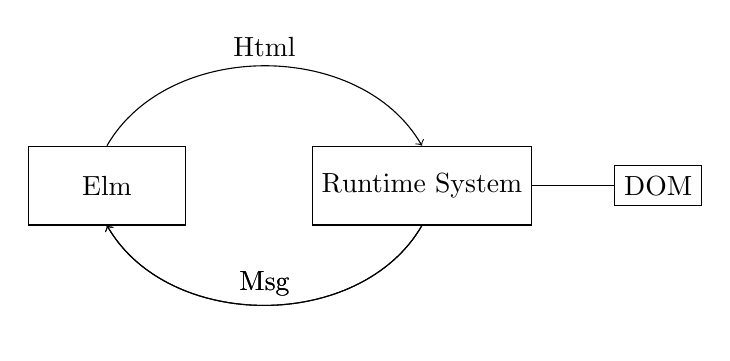
\begin{tikzpicture}
  % Nodes
  \node (p) [rectangle, draw, minimum height=1cm, minimum width=2cm] at (0, 0) {Elm};
  \node (i) [rectangle, draw, minimum height=1cm, minimum width=2cm] at (4, 0) {Runtime System};
  \node (d) [rectangle, draw, minimum height=0.5cm, minimum width=1cm] at (7, 0) {DOM};
  % Arrow
  \draw[->] (p.north) to[out=60, in=120] node[midway, above] {Html} (i.north);
  \draw[->] (i.south) to[out=-120, in=-60] node[midway, above] {Msg} (p.south);
  \draw[->] (i.south) to[out=-120, in=-60] node[midway, above] {Msg} (p.south);
  \draw[] (i) -- (d) node[midway, above] {};
  % Header
\end{tikzpicture}

  \caption{Elm Architecture (Figure adapted from \cite{elmFig})}
  \label{fig:elmArchitecture}
\end{figure}

\subsection{Module Architecture}

In this application, the Elm-box is a module, while the runtime system, is the
core itself. The core invokes all modules, all of which, should have these three
functions, \lstinline{init}, \lstinline{update}, and \lstinline{view}.

\paragraph{Init} Returns a collection of key-value-pairs, which represent
the state of the core.

\paragraph{Update} Returns a collection of key-value-pairs, which
overwrite existing key-value-pairs in the state, or are appended to the state.
Invoked every time a \textit{Msg} is sent.

\paragraph{View} Returns a collection which represents \gls{html},
which is rendered by the core.

\begin{center}
  \lstinputlisting
    [ language=Haskell
    , caption={Module Type}
    , label=lst:pluginExample
    ]{./code/plugin-example.hs}
\end{center}

A module is initialized by invoking the \textbf{init} method, which returns a
state. This can be seen in figure \ref{fig:moduleInit}. After the state
initialization, the modules' \textbf{view} method is invoked, which initializes
the \gls{ui} for the user, which can be seen in figure \ref{fig:moduleInitView}.

\begin{figure}
  \centering
  \input{./figures/plugin-init}
  \caption{Module state initialization stage}
  \label{fig:moduleInit}
\end{figure}

\begin{figure}
  \centering
  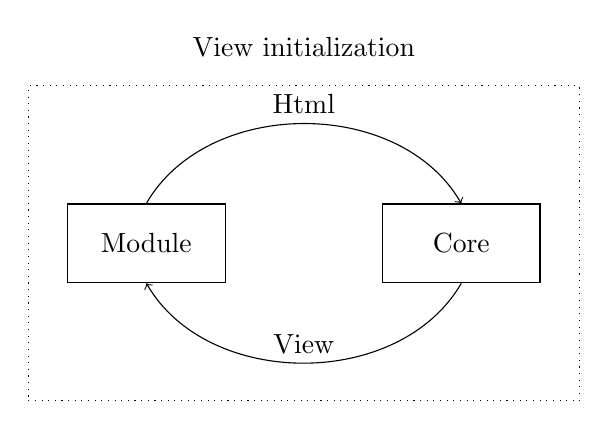
\begin{tikzpicture}
  \node [rectangle, draw, minimum height=4cm, minimum width=7cm, dotted] at (2, 0) {};
  \node [] at (2, 2.5) {View initialization};

  \node (i) [rectangle, draw, minimum height=1cm, minimum width=2cm] at (4, 0) {Core};
  \node (p) [rectangle, draw, minimum height=1cm, minimum width=2cm] at (0, 0) {Module};
  \draw[->] (p.north) to[out=60, in=120] node[midway, above] {Html} (i.north);
  \draw[->] (i.south) to[out=-120, in=-60] node[midway, above] {View} (p.south);
\end{tikzpicture}

  \caption{Module view initialization stage}
  \label{fig:moduleInitView}
\end{figure}

\todo{Explain the module architecture in IDE terms, so with IDE examples}

Since the \gls{ide} is written in both TypeScript and Rust, a method of encoding
type information when crossing between the TypeScript and Rust environment was
needed. It was achieved by simply typing \gls{json} objects, so while the state
could be represented as any \gls{json} object, it was instead represented as
nested \gls{json} objects, where, all values, except \textbf{null}, where
encoded as an object with one field, being the type of the object, and then the
value. So an int would be \textbf{\{ int: 0 \}}.

The reason for representing a JSON object as key-value pairs, is that this could
be easily translated to a Rust representation of the same type, using the
\textit{Serde} crate. This allows for creating Rust structs which represents
JSON objects, and creates an automatic encoder/decoder between Rust and JSON.
This ensures a good cooperation between the \textit{frontend} and
\textit{backend}.
\todo{Rewrite}

The general idea was that for each possible \gls{dom}-event, there would exist a
way to send a Msg. Each Msg contains a Msg name, and some value, which enabled
pattern matching on Msg, similar to Elm, for modules, so each module could
choose to act on a Msg or not.

In listing \ref{lst:pluginCounterExample}, an example of a counter module can be
seen. This module initializes a state, containing the field \textbf{"counter"},
with the value \textbf{VInt 0}.

The \textit{update} function the module exposes, matches on a \textbf{"counter"}
msg, with a \textbf{VInt i} value. If the given Msg matches this, then the
module adds to the \textbf{"counter"}-field, the value from the Msg, which is
$1$.

Finally, the \textit{view} function renders a button, which when pushed by a
user, sends the \textit{counter-Msg}.

\begin{center}
  \lstinputlisting
    [ language=Haskell
    , caption={Module Architecture}
    , label=lst:pluginCounterExample]{./code/plugin-counter-example.hs}
\end{center}

\subsubsection{Module purity}

One important thing in this architecture, is the pureness of module. The state
of a module needs to be kept in the core application, and not in the module
itself. The reason for this is twofold. It allows for the possibility of the
core to be optimized in the future, as modules which do not react to a certain
msg-state combination, can be noticed, and ensure modules are not unnecessarily
invoked. It also lowers the complexity for module developers, as it is easier to
reason about modules if \textit{all} they do is read or write to some state.

If we have the modules $A$ and $B$, where their relationship is $A \to B$,
meaning $A$ \textit{invokes} $B$ by sending some Msg, which $B$ reacts too, and
we want something to happen before $B$ reacts, we can add a new module, $C$,
which also reacts to the same Msg, but if we know the name of the module $B$,
we can set the name of module $C$ to be \textit{above} the order, relative to
$B$, ensuring that $C$ always triggers before $B$.

But this introduces a possibility for some hierarchy in the module ecosystem.
For example, a module could act as a framework, and therefore needs to only be
loaded once, creating new locations, with styling.

\subsection{Module v2 Cons}

\subsubsection{Module v2 cons}

\todo{Sum up all the issues with this architecture}

\begin{enumerate}
  \item React sucks
  \item Modules cannot invoke modules
  \item Slow
  \item Not asynchronous
  \item Ever growing state
\end{enumerate}


With this setup, however, the state is appending/overwriting -only, which means
the state can only grow.

This setup is also not really modular, as a single module cannot invoke another
module without being impure. The only way to invoke/trigger another module, is
to throw a \textit{Msg}, which would trigger an update -> view -> cycle. So
a module cannot \textit{listen} for a single message, all modules are triggered
by the same \textit{Msg}, and handled accordingly.

\subsubsection{State Collision} \label{sec:collision}

A state collision occurs when two or more modules updates the same field, during
the same update-cycle. This issue also occurs when folding two states.

Was \textit{solved} with this:

\begin{center}
  \lstinputlisting
  [ language=Haskell
  , caption={State Collision Typing}
  , label=lst:stColType
  ]{./code/state-collision-types.hs}
\end{center}

Takes list of states from all modules, checks for collisions. It returns a
list of
\lstinline[language=Haskell]{Either [(String, State)] ([(String, State)], String)}.
If it is a collision, then it's a
\lstinline[language=Haskell]{Right ([(String, State)], String)}, which is a
tuple where the first element is a list of tuples, being the module and their
state, and the last element being the field that the collision occurred on.
The other value: \lstinline[language=Haskell]{Left [(String, State)]}, are the
module state that has no collision.

\paragraph{Collision} A collision between two states occurs if they share the same
field.

There are several different ways to correct a collision between two
states:

\begin{enumerate}
  \item If the states are of same type:
    \begin{enumerate}
      \item If the value from one of the colliders are unchanged from the previous state:
        \begin{enumerate}
          \item Keep the new value OR Keep the old value
        \end{enumerate}
      \item Else
        \begin{enumerate}
          \item Apply the types' semigroup operator to the fields.
        \end{enumerate}
    \end{enumerate}
  \item Else
    \begin{enumerate}
      \item If the value from one of the colliders are unchanged from the previous state:
        \begin{enumerate}
          \item Keep the new value OR Keep the old value
        \end{enumerate}
      \item Else
        \begin{enumerate}
          \item Keep the left-hand side value OR Keep the right-hand side value
        \end{enumerate}
    \end{enumerate}
\end{enumerate}

Since the states are ordered by the name of the module they come from, we
have a consistent ordering of left-hand side and right-hand side. If the same
modules give a collision on the same input, (given that all modules are pure), the
resulting state will be the same every time. The problem is that applying some
function on the values could be an unwanted way to resolve collisions. The
standard way will be to log the collision, and then drop both states. Even
if two states have A and B amount of fields, and just one collision, we will
drop A + B amount of fields. Therefore, a module developer should avoid
collisions.

\begin{center}
  \lstinputlisting
  [ language=Haskell
  , caption={State Collision}
  , label=Listing
  ]{./code/state-collision.hs}
\end{center}

\todo{Mention how updating two fields on the same object also counts as a collision}

This problem of resolving state collision only occurs because each module
returns a subtree of the state. We then have to analyze the new coalesced tree
for each new subtree that is added, to figure out if there occurs any collision.
And then notifying the module developer of which field this collision occurred
on, and which modules tried to modify that field.

\section{Module V.3} \label{sec:mod3}

The third and hopefully final, plan:

\begin{enumerate}
  \item Everything is a module
  \item Modules can \textit{invoke} modules
\end{enumerate}

A module only exposes two functions:

\paragraph{Init} Returns nothing

\paragraph{Handler} Returns nothing

In the previous architecture version, each module directly changed the state,
which caused issues. Instead, each modification a module does, \textit{acts}, as
a direct modification, but is in fact, translated to a DSL which can be analyzed
for possible collisions. This was discovered to be a need, as in the new
version, the \gls{ui} was also restructured, to allow for less re-rendering, and
this restructuring, made it clear that changing the state, or changing the
\gls{ui} is just tree manipulations, which will be discussed more later.

\subsection{Zero core architecture and microservice architecture}

The new plan came with a change of viewpoint. Think of
\textit{everything being a module}, this pushed for a modularization between the
then tightly coupled parts, the \textit{frontend} and \textit{backend}. As
mentioned, having two different languages could allow for easier support of
modules written in different programming languages, but for this to work in an
optimal way, both the \textit{frontend} and \textit{backend} should be loosely
coupled. This is an equivalent architecture to microservices.
\todo{Add diagrams and examples}
\todo{Mention runtimes}

\subsection{Vanilla TypeScript}

Instead of using React as the frontend framework, TypeScript was chosen, which
simplified the integration between the backend and frontend, as the complexity
of React's state management could be avoided, along with React's hydration.
Given the rendering was now more \textit{hands-on}, the core could expose a lot
of the functionality for rendering, which modules could change. This would
increase the difference between the \gls{jsms} and \gls{rsms}, as the backend
was not privy to this API, but this was not seen as an issue, as this API would
turn module non-pure.
\todo{Mention pureness earlier}

\subsubsection{Removing abstractions}

It became prudent, due to the change of architecture, to change the entire
frontend, moving away from React, and using \textit{bare-bones} TypeScript. This
would enable easier integration into the \gls{jsms}.

\subsection{Core Modifications}

Learning from the issues outlined in section \ref{sec:collision}, instead of a
module returning the new core, it will rather return a set of instruction on
\textit{how} the core is to be modified, resulting in what the module developer
wants the core to be. The reason for turning it around in this manner, is that,
the new architectural change also came with a change on how the \gls{ui} is
modeled, as it is now up to the core to figure out an inexpensive way to do
rendering. Since the core has \gls{ui}-structure which is a representation of
what the \gls{dom} should be, it can be treated as a Virtual-\gls{dom}, similar
as to how React does it. This also means that there could be a collision on
\gls{ui}-change, as well as on a state-change. Instead of solving the equivalent
problems twice, it was decided to try to treat the issues with collisions in
state and \gls{ui} as the same issue; its some form of tree-manipulation.

\begin{center}
  \lstinputlisting
    [ language=Haskell
    , caption={Core}
    , label=lst:coreAdt
    ]{./code/module-example-core.hs}
\end{center}

In listing \ref{lst:moduleEvent}, one can see the structure of an
\lstinline[language=Haskell]{Event}. This allows for modules to
pattern match on specific \lstinline[language=Haskell]{Event}s, and as in the
previous version, only react to specific \lstinline[language=Haskell]{Event}s.
What is different, is as shown in the \ref{lst:moduleCounter} listing, is that
each module registers an \lstinline[language=Haskell]{EventHandler} which is
\textit{only} invoked when the specific \lstinline[language=Haskell]{Event} it
is registered with, is called. This ensures a more direct form of
module-to-module communication, as a module can directly \textit{invoke} another
module. This changes the structure of the module architecture to go from one
wherein the core is a terminal object, to a more \textit{complicated} one, in
which module families can form.

\begin{center}
  \lstinputlisting
    [ language=Haskell
    , caption={Module Event Type}
    , label=lst:moduleEvent
    ]{./code/module-example-event.hs}
\end{center}

\begin{center}
  \lstinputlisting
    [ language=Haskell
    , caption={Module Counter Example}
    , label=lst:moduleCounter
    ]{./code/module-example-counter.hs}
\end{center}

\begin{center}
  \lstinputlisting
    [ language=Haskell
    , caption={Module Counter Example Event Handler}
    , label=lst:moduleEventHandler
    ]{./code/module-example-counter-handler.hs}
\end{center}

The module example shown in listing \ref{lst:moduleCounter} and
\ref{lst:moduleEventHandler}, is again, a simple counter example, where the
module registers a \lstinline[language=Haskell]{CoreModification}, changing the
UI-hierarchy, by adding a button which throws an
\lstinline[language=Haskell]{Event} that is handled by the
\lstinline[language=Haskell]{EventHandler} shown in
\ref{lst:moduleEventHandler}, which again, modifies the core by changing the
counter field with the value from the \lstinline[language=Haskell]{Event}.

\subsection{Tree Manipulation}

\todo{
  Mention Magnolia here, and how the satisfaction/unit test thing can "prove"
  this
}
This restructure changes the way the view is rendered. Instead of the view being
re-rendered for each state-update, the view, or \gls{ui}-hierarchy, is only
\todo{Mention earlier how React was used/considered due to the "smart" re-rendering}
modified by modules. This modification is similar to the earlier state
modification, so a unified algorithm to solve this can be used. If there is an
easy way to translate a \gls{ui} modification to a state modification, and back
again. To solve this, instead of having a module return the actual
modifications, meaning, the updated core, a module returns a set of instructions
of what to do with the core.

\begin{center}
  \lstinputlisting
   [ language=Rust
   , caption={Instruction (Rust)}
   , label=lst:inst
   ]{./core/src-tauri/core-std-lib/src/instruction.rs}
\end{center}

The listing \ref{lst:inst}, shows of how the \textbf{Instruction}-set makes the
modification of the core, a kind of group, as given the definition
\ref{def:group}, we can construct one:

\begin{theorem}[Instruction Group]
  Let $\Sigma$ be the set of all strings, $Val$ be the set of all
  \textbf{Values}, $Html$ be the set of all \textbf{Html} variants, and
  $Inst_{val}$ be the set of all \textbf{Instruction} defined as:
  $$
    NoOp = \left \{ noOp \right \}
  $$
  $$
    NoOp \in Inst_{val}
  $$
  $$
    Add_{val} = \left \{ (x, y, z) \vert x \in \Sigma, y \in \Sigma, z \in Val \right \}
  $$
  $$
    Add_{val} \in Inst_{val}
  $$
  $$
    Rem_{val} = \left \{ (x, y, z) \vert x \in \Sigma, y \in \Sigma, z \in Val \right \}
  $$
  $$
    Rem_{val} \in Inst_{val}
  $$
  $$
    Then_{val} = \left \{ (x, y) \vert x, y \in Inst_{val} \right \}
  $$
  $$
    Then_{val} \in Inst_{val}
  $$
  For any $x \in Add_{val}$ there exist a unique $y \in Rem_{val}$, such that:
  $$
    x \oplus y = noOp
  $$
\end{theorem}

This, unfortunately, cannot be encoded in Rusts type system, but when implementing
$combine$, we can map the variants along with the specific fields being added
($Add$), modified ($Mod$), or removed ($Rem$), to get a more optimized
instruction set. If we are modifying a value on field $foobar$, but in the same
instruction set, remove it, then the modifying instruction is an $NoOp$.

\todo{Add trivial module example, or something}

Using this as a module developer is quite abstract, so to facilitate development
of modules, a helper class was created, which \textit{translates} modifications
to instructions. As shown in listing \ref{lst:ui-builder} and
\ref{lst:state-builder}, a module developer simply invokes different methods on
the builder, eventually building a \textbf{CoreModification}, to be sent.

\begin{center}
  \lstinputlisting
   [ language=Rust
   , caption={UI Builder (Rust)}
   , label=lst:ui-builder
   ]{./code/module-ui-builder.rs}
\end{center}

\begin{center}
  \lstinputlisting
   [ language=Rust
   , caption={State Builder (Rust)}
   , label=lst:state-builder
   ]{./code/module-state-builder.rs}
\end{center}

This allows for an ergonomic way for module developer to create modifications on
the core, without having to understand the syntax of the
\textbf{Instruction}-set.

\begin{center}
  \lstinputlisting
   [ language=Haskell
   , caption={Module Type}
   , label=lst:moduleType
   ]{./code/module-example.hs}
\end{center}

As one can see in listing \ref{lst:moduleType}, a module only exposes its name,
and an \lstinline[language=haskell]{init} function, which takes the
\lstinline[language=haskell]{Core}, which is a representation of
the core application shown in listing \ref{lst:coreAdt}.

\subsection{Backend Agnostic Frontend}
\todo{This is not true anymore}

As mentioned in the previous section, the tech stack splits the application into
two, loosely coupled parts. The \textit{frontend} and \textit{backend}. This
architecture does facilitate the concept of an agnostic frontend. That is, if,
as is the case per the previous plan, all logic pertaining to the core is in the
\textit{frontend}, cannot the backend be anything, as long as it fulfills the
following criteria.

\subsection{Making the Core evaluate modifications asynchronously}

Due to Rust first class focus on concurrency, it was trivial to make the core
modifications run asynchronously. In previous iterations, the core evaluated
one event at a time, waiting until all modules had finished their computations,
before emulating the change and allowing for the next event to be evaluated. But
this caused a noticeable \textit{lag} if an event was long. This was solved by
changing the core modification evaluation from a simple method to be invoked, to
an \gls{mpsc} channel system. Using \textit{tokio}, a Rust crate for
asynchronous development, a channel for core modifications was created, and
instead of the core collecting all modifications, each module is invoked and
\textit{awaited} for in a separate thread, where in each module, if they have a
core modification, sends the modification to the core channel, which works on
a first come, first server basis. Here the core can evaluate the changes, also
on a separate thread.
\todo{Mention in v2 how file system stuff made stuff sluggish}

\begin{itemize}
  \item File system modification
  \item Module loading
\end{itemize}

\section{Testing} \label{sec:testing}

\todo{Showcase example of testing the ide}

A zero-core application is equivalent to a microservice architecture, in that
testing is important to ensure changes in one module does not inadvertently
affect another.

\subsection{Mocking}

Due to the \textit{pureness} of modules, mocking can be achieved easily, and
therefore, modules can be tested alone, which is good, because testing a
singular module is inexpensive.

\subsection{Unit Testing}

A module developer should create unit tests for their module. This can easily be
done, and tested many times, due to the light-weightiness of a module.

\subsubsection{UI Testing}

\todo{Mention of ui testing is part of unit testing}

\subsection{Module Family Testing}

If a module changes some feature, let's say in the editor functionality, the
module family tree encompassing this functionality needs to be tested, to ensure
nothing breaks.

\subsubsection{Contract Testing}

As a module developer, on is designing some kind of \gls{api}, but the developer
has no say in how a consumer of the \gls{api} consumes it. In a microservice
architecture, the common way to work around this, is to version control the
\gls{api} by prefixing \textit{v*} in front of all endpoints in the \gls{api},
where star, (*), is the version of the \gls{api}. This way, the \gls{api}
designer can develop new \gls{api}s, without worrying about breaking
functionality that consumers of the \gls{api} depend on. This, however, usually
means having to maintain equivalent \gls{api}s in parallel, until one decides
to deprecate an older less used version, forcing consumers to move on to the
newer version of the \gls{api}.

Instead of relying on such a versioning system, module developers could use
\textit{contract testing}.

\paragraph{Contract Testing} Imagine some \gls{api}, and several consumers,
$A, B, C$, The \gls{api} developer is serving some data, in this case an
integer number, which all the consumers use. One day, the developer finds out
that using integers is not optimal, and want to move on to using floating point
numbers instead. Changing the \gls{api} outright could bring issues, as the
consumers might rely on the \gls{api} being an integer, instead of a float. But
the change is needed, or wanted, at least. In this scenario, it is \textit{easy}
to inform all the consumers of the \gls{api}, but if the consumer count
increases tenfold, this is more difficult. A notice can still be sent, but it is
not feasible to ensure all consumers commit time to change their ways. Contract
testing ensures that, if a change like this occurs, the maintainer of the
\gls{api} is notified by which consumer this change breaks.

The issue is to create these contracts. Using frameworks like Pact \cite{pact},
a developer creates a \gls{dsl} test, where they describe how the provider or
consumer reacts to certain interactions. But since everything is a module, we
can automate this.

\subsection{Automating Contract Testing}

This process could be partially automated, as all modules have to register the
event they want to handle. Furthermore, all events thrown are also explicitly
done through the core instance, meaning a \textit{test-core} could be created,
which registers which event is thrown from what module, and all dependencies
between modules can be noted.
\todo{Implement this}

\subsection{End-To-End-Testing}

The final step in the testing pipeline, is to test the entire application
together. This is known as \gls{e2e}, but this is expensive.

\section{Modules}

\todo{Introduction}

Here are some examples of modules implemented using the proposed architecture.

\subsection{Magnolia Dependency Graph Visualizer}

\todo{Implement and showcase this module}

\subsection{IDE Module Family}

\todo{Showcase the modules created to have a rudimentary IDE}
\todo{Mention QOF modules for future module developers}
\todo{Mention Project Management}

\subsection{Caching}
\todo{Properly implement this}
In Magnolia, caching of \gls{lsp} queries is important. And caching of the
compiled code.

\subsection{Editor Module Family}

\todo{Implement a rudimentary editor}

\subsection{Magnolia Language Server}

\todo{Implement a rudimentary Magnolia LS}


\chapter{Related Work} \label{cha:related}

\section{Existing module architectures in IDEs}

There exists module architectures in other \gls*{ide}s.


\subsection{Eclipse}

\gls*{ide}s are one of the most common application that supports extensions by
third-party code. \gls*{ide}s like \gls*{eclipse} and \gls*{intellij} are
specialized for working with Java, but they can still support other languages
with the help of modules. A module in \gls*{eclipse} for instance, could extend
\gls*{eclipse} with functionality like syntax highlighting, code completion,
Go-to-definitions, debugging, and more, for standard programming languages.
A lot of this functionality, comes from module-to-module extension, as in
\gls*{eclipse} modules can extend modules, with the use of the \gls*{erpc}~\cite{eclipseRcp}.

\subsubsection{Eclipse Rich Client Platform}
\*gls{erpc} is a platform for building desktop applications. \gls*{eclipse}
being an example of this platform in action. A plug-in could for example be
responsible for setting up the general \gls*{ui} layout, similar to our module,
\textit{ide\_framework}, and another plug-in could then modify this \gls*{ui} by
adding a file explorer, similar to our module \textit{ide\_explorer}.


\subsection{NetBeans}

An important part of NetBeans core architecture, is the NetBeans Module
\gls*{api}. This \gls{api} is responsible for supporting the
\textit{runtime environment}, which is the minimum amount of modules needed to
run the NetBeans application. A module in NetBeans is a JAR file, in which a
module can, amongst other things, list their public packages. This means that
other modules can directly invoke methods provided by this package.


\subsection{IntelliJ}

The extensibility \gls*{intellij} has, is achieved by its extensions points
architecture. This is an \gls*{api} for plugins to integrate with the
\gls*{ide}. Plugins use this \gls*{api} to register their implementations.

\subsection{Visual Studio}

There are two kinds of extensions in Visual Studio, \textit{VSPackage} and
\textit{MEF} extensions. \textit{VSPackage} are mainly used to extend
functionality like tool windows and projects, while \textit{MEF} extensions are
used to customize the text-editor.

\subsection{Visual Studio Code}

\gls*{vscode} is an extensible \gls*{ide}. It achieves this extensibility with
its extension \gls*{api}. This \gls*{api} allows for extensions to modify the
look and behavior of the \gls*{ide}. In fact, many of the core \gls*{ide}
features are possible due to built-in extensions.

\subsection{Emacs}

Emacs\footnote{\url{https://www.gnu.org/software/emacs/}} is an extensible text
editor. Almost all of Emacs functionality is achieved by writing code in Emacs
Lisp, a dialect of Lisp\footnote{\url{https://lisp-lang.org/}}. Unlike other
\gls*{ide}s, Emacs does not restrict modules to a certain \gls*{api}, instead
they are free to modify anything, as the functionality from the Emacs Lisp,
\textit{sits} atop of a core written in C, which abstracts away platform
specific code, and enables Emacs to be turned from an a \textit{simple} text
editor, to write and send emails, multimedia management and much more.


\subsection{Theia}

\say{The Theia \gls*{ide} is a modern \gls*{ide} for cloud and desktop built on the Theia Platform}\footnote{\url{https://theia-ide.org/}}.

Eclipse Theia is a highly extensible \gls*{ide}, supporting \textit{extensions}
from \gls*{vscode}, their own extensions and plugins, and \textit{headless}
plugins. Theia differentiates between extensions and plugins, where a
plugin is installed during runtime, and an extension is installed during
compile-time.

Theia reuses components from \gls*{vscode}, like their extensions \gls*{api},
which enables them to support \gls*{vscode} extensions. Theia plugins share
similarities with \gls*{vscode} extensions, but are not restricted to
\textit{just} the \gls*{vscode} \gls*{api}.

Theia's extensions are designed to add or remove existing core functionality in
Theia. They also have access to the entire core \gls*{api}.

An headless plugin runs without access to the frontend, meaning they are suited
for \gls*{cli} interactions, or similar use cases where a frontend is not
needed.

Theia is both a desktop \gls*{ide} and a web \gls*{ide}. Where there is no real
distinction between the two, both abstracting it to a frontend and backend. This
is similar to our zero-core \gls*{ide}, as we can make this abstraction due to
our usage of a web view for the desktop \gls*{ide}.


\section{Multi-way Dataflow Constraint System} \label{sec:mdcs}

One thing this application does not provide a solution for, is the difficulty
in designing good \gls*{gui}. Following the \gls*{mvc}-pattern, \gls*{gui}s can
represent structures such as lists, which users might want to manipulate in
some fashion, like appending or rearranging the items in the list. Managing such
a change, especially one that involves \gls*{gui} widgets can be a challenge,
since a change in the view should be reflected in the model, and encoding this
can be very involved. Luckily, there exists frameworks that make this task
easier. \textit{WarmDrink},~\cite{warmDrink, dslMdcs} is a JavaScript
framework that allow a developer to declarative specify structural changes in
an application. This can be achieved, since the \gls*{ide} exposes a simple
\gls*{api} for runtime systems. A runtime system specifically for a \gls*{mdcs}
could be implemented for JavaScript modules. This could also be done for the
Rust modules, by utilizing the crate developed by Svartveit~\cite{mcdsRust}.
The module developer experience is important, so it's good that there exist
\gls*{mdcs} tooling to ease a module developers experience~\cite{toolMcds}.

Another issue in \gls*{gui}s is optimizing performance in regard to events
triggered by user actions, such as scrolling, resizing or typing. These events
could happen many times in a second, while in theory user speed is trivial for a
computer to keep up with, there are instances where a module family could be
quite large, meaning many different modules are triggered by the same event many
times. There are techniques, called event coalescing, for handling this, like
debouncing and throttling.

\paragraph{Debouncing} Debouncing is a technique where you delay the sending of
an event until after some time period $T$ has passed. Once the event is triggered
$T_0$ starts counting down. If the same event is re-triggered while $T_0 > 0$,
$T_0$ is reset by $T_0 = T$. If $T_0 = 0$, then the event is sent. Ensuring that
$T$ is not too large, is important, as if $T$ is above some threshold, the user
of the \gls*{gui} will notice, and it will make the application \textit{feel}
slow.

\paragraph{Throttling} Throttling is a similar technique to debouncing, except
instead of delaying the event by some time $T$, the event is only sent when
$T_0 = 0$. Meaning the event is sent at regular intervals, and could be sent at
the exact same point in time when the user triggered the event, or it could
happen at most, $T$ units after the user action.

Debouncing and throttling work in less complex \gls*{gui} structures, but as the
amount of features in an application increases, the complexity will also
increase. These event-coalescing-strategies are a source of subtle bugs, as
event coalescing can easily break modularity. In a \gls*{jsms}, this issue could
be solved by using \textit{flushable promises}~\cite{flush}. This could have
solved our issue, where we had some Event handler that took noticeably longer
time to return, but since this was a Rust-Module, we could \textit{solve} this
by doing this computation on another thread. If it was a JavaScript module we
could have solved it by using \textit{flushable promises}.

If we implement a \gls*{ls}-client in JavaScript, \textit{flushable promises}
could allow for a smoother experience, as things like \textit{looking up}
renaming in a Magnolia project is a more involved process for the compiler,
and in larger projects, could take a noticeably long time.


\section{Automated testing}

Due to the extensive modularity of the application, all modules can be tested
individually, by \textit{mocking} the expected state and events. This means that
breaking changes in one module can be detected before \gls*{e2e} testing, which
is expensive. But this can only verify the general logic of a module and module
family, not the UI. To achieve such automation, one could rely on an automated
testing framework, like the one in~\cite{autoUi}. Or if one is working with a
\textit{simple} JavaScript runtime, one could use third party software like
\textit{Playwright} for creating tests, as it can auto generate the \gls*{dsl},
while the developer uses the module or entire \gls*{ide} if it is an \gls*{e2e}
test. This would help a module developer to discover behavior that a user might
not expect~\cite{leastGui}.


\section{Syntactic Theory Functor}

\gls*{stf} is a framework for creating, reusing and restructuring
specifications\cite{stf:haveraaen:2020}, specifications from algebraic
specification languages like CafeOBJ~\cite{cafeObj}. \gls*{stf}s are also used
by the new Magnolia compiler\footnote{As of May 2025, still in development}, to
resolve renaming in Magnolia and \textit{flattening} of the \gls*{asr} to be
shown to the developer \cite{wiig}.


\section{Abstract algebra}

Magnolia is a kind of algebraic specification language, like CafeOBJ~\cite{cafeObj}.
An algebraic specification language, is a language where one can develop
similarly as to how one might create an algebraic structure. As shown in the
development of this \gls*{ide}, this can be quite useful way of thinking.


\section{Language workbenches}

Language workbenches are environments for simplifying the creation and use of
computer languages~\cite{lwb}.


\section{Language Server}

The most important features in a modern \gls*{ide} are possible due to the
\gls*{lsp}. \gls*{lsp} is a protocol for a language server and editor,
(the client), in which they communicate, allowing for many of the features
mentioned in section \ref{sec:ide}, and explicitly mentioned in table
\ref{tbl:ide}. \gls*{lsp} being the standard since the 2020s, is a sign of
modularity being preferred, as now a single \gls*{lsp} can be created, and used
across several different applications, like IntelliJ, VS Code and \gls*{vim}.
While useful for \textit{standard} language, this is the limiting factor when it
comes to supporting experimental languages, as not only does a new set of
protocols need to be appended to a language server, the editor itself needs to
be changed to actually use these protocols. This creates a lot of work, for both
the \gls*{ide} developer and for the compiler developer. Here is where a modular
approach can help both. If some new functionality or feature is added to the
experimental language, this off course means the compiler/interpreter has to be
expanded and/or modified, but for the \gls*{ide}, a module could be added and/or
modified to utilize this change, instead of having to change the entire
application.

\begin{table}[]
  \centering
  \caption{\gls*{ide} features enabled by \gls*{lsp}}
  \label{tbl:ide}
  \begin{tabular}{|l|l|}
    \hline
    IDE Feature & \gls*{lsp}-method \\ \hline
    Go to Declaration & textDocument/definition \\ \hline
    Go to Implementation & textDocument/implementation \\ \hline
    Auto-completion & textDocument/completion \\ \hline
    Hover & textDocument/hover \\ \hline
    Warnings & textDocument/publishDiagnostics \\ \hline
    Rename & textDocument/rename \\ \hline
  \end{tabular}
\end{table}

An example of this in action, say a developer is working on a file
\textit{main.ts}, in their Typescript project. They hover over a type imported
from, and defined in \textit{types.ts}. This is what happens:

\begin{enumerate}
  \item The editor detects the user is hovering over a \textit{special} word
  \item The editor sends a request to the Typescript \gls*{ls}
  \item The \gls*{ls} responds
  \item The editor formats the response into a small window showcasing the
    documentation and implementation of the type
\end{enumerate}


\chapter{Conclusion} \label{cha:conclusion}

The hypothesis \ref{hyp:modular} is right, source? Me.

\section{Modular Development}

In this thesis, we have shown that developing against a zero-core modular
architecture is trivial. By utilizing seperation of concerns, a module developer
need to only understand the feature they want to extend, or if it is an entirely
new feature, find out what has been done before.

\section{Making an IDE is hard}

An \gls{ide} has many features, which are needed to enhance the developer
experience. To achieve this, the modular approach enables future users to
enhance the application.

\begin{figure}
  \centering
  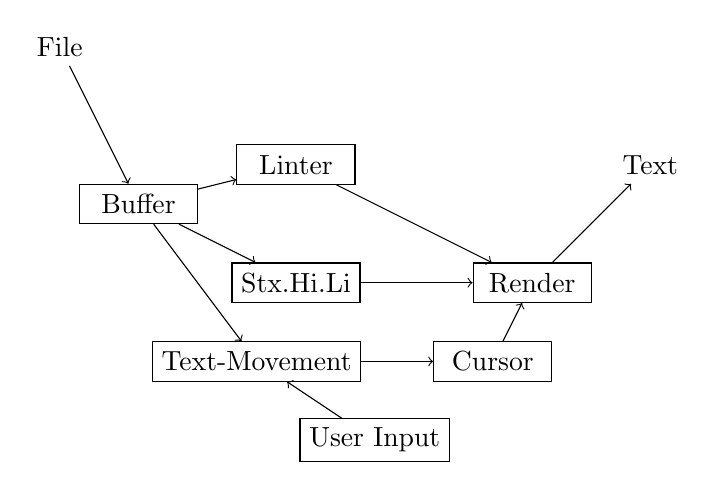
\begin{tikzpicture}
  % Nodes
  \node (file) [] at (-6, 3) {File};
  \node (parser) [rectangle, draw, minimum height=0.5cm, minimum width=1.5cm] at (-5, 1) {Buffer};
  \node (stxhili) [rectangle, draw, minimum height=0.5cm, minimum width=1.5cm] at (-3, 0) {Stx.Hi.Li};
  \node (text-movement) [rectangle, draw, minimum height=0.5cm, minimum width=1.5cm] at (-3.5, -1) {Text-Movement};
  \node (linter) [rectangle, draw, minimum height=0.5cm, minimum width=1.5cm] at (-3, 1.5) {Linter};
  \node (cursor) [rectangle, draw, minimum height=0.5cm, minimum width=1.5cm] at (-0.5, -1) {Cursor};
  \node (user-input) [rectangle, draw, minimum height=0.5cm, minimum width=1.5cm] at (-2, -2) {User Input};
  \node (render) [rectangle, draw, minimum height=0.5cm, minimum width=1.5cm] at (0, 0) {Render};
  \node (text) at (1.5, 1.5) {Text};
  % Arrow
  \draw[->] (file) -- (parser) node[midway, above] {};
  \draw[->] (parser) -- (stxhili) node[midway, above] {};
  \draw[->] (parser) -- (linter) node[midway, above] {};
  \draw[->] (parser) -- (text-movement) node[midway, above] {};
  \draw[<-] (render) -- (stxhili) node[midway, above] {};
  \draw[<-] (render) -- (linter) node[midway, above] {};
  \draw[<-] (cursor) -- (text-movement) node[midway, above] {};
  \draw[<-] (text-movement) -- (user-input) node[midway, above] {};
  \draw[->] (cursor) -- (render) node[midway, above] {};
  \draw[->] (render) -- (text) node[midway, above] {};
\end{tikzpicture}


  \caption{Text Editor Module Family}
  \label{fig:extendedModuleFamily}
\end{figure}

In the figure \ref{fig:extendedModuleFamily}, the \textit{cursor} is the place
at which text is placed when the user writes. If the user clicks someplace in
the document, the cursor \textit{jumps} to that place. If the user uses the
arrow-keys to move around, the cursor moves one character to left or right, or
one line up and down, depending on which arrow-key was pressed.

\section{Cons}

If you are the one developing every module, it get's very complex.

If you have a problem, and try to solve it with concurrency, now problems two
have you.

\chapter{Future Work} \label{cha:future}

Would've, could've, should've.


\section{Technical debt}

It just piles and piles and piles on.

\begin{enumerate}
  \item Missing tests
  \item Not a total mapping between \gls*{dom} stuff and the Rust counterpart
  \item Inconsistent \gls*{ui}
\end{enumerate}


\subsection{Testing}

No unit tests for the TypeScript side, no integration testing between the
frontend and backend.

There should be tests made to ensure that a module behaves the same, if written
in Rust or JavaScript. This can be an issue, because the way a module interacts
with the \gls*{ide} is through a core, which is implemented separately for the
different module systems. Test modules should be made, ensuring that the end
state of the \gls*{ide} is the same, when the module does the same action. But
this would require the modules being semantically the same for the different
test cases. In any case, difficult to ensure all edge cases have been covered.

\subsection{Language agnosticism}

Steps should be made to mitigate the shortfall of this solution, with regard to
language agnosticism. The differences in installation for \gls*{rsms} and
\gls*{jsms} are mainly due to how trivial it is to install JavaScript modules,
compared to Rust modules. \gls*{jsms} should enforce a similar system of module
building as \gls*{rsms}, not only to ensure less semantic differences, but also
to ensure safety, as restricting the \gls*{jsms} is good.

\subsection{Attribute and instructions}

Can't remove or change eventListeners currently. This is because to remove an
EventListener, the exact same function passed to the \textit{addEventListener}
must be used, which means a reference to this function needs to be stored, but
having two or more of the same type? It can get confusing for a module developer
of what should actually happen.

\subsection{Keypresses}

A common feature of \gls*{ide}s is being able to have certain keybindings for
different actions. For example, in \gls*{vscode}, one can hit \textit{CTRL}
$+$ \textit{n} to open up a new tab, with a new file. This system is not yet
possible in the \gls*{ide}, but this is due to a lack of a supporting module
family. But, given that this is a common feature in \gls*{ide}s, this should be
a priority.

\subsection{Inconsistent UI}

Difficult to keep the \gls*{ui} representation consistent with the \gls*{dom}.
An example of this, is that the \gls*{ui} representation in the \gls*{ide} does
not store information like the possible \textit{value} an \gls{html} might
have. So for the editor module, there is no efficient way to know what text is
in the editor. Another example, is for the module installer, there is no way for
the module to \textit{query} the \gls*{ui} for information about the form it
presents the user, seeing what values are in the fields. A workaround to this
was used, where depending on what element an \textit{eventListener} was added
to, the sent event would be \textit{sticky}, meaning it would add extra
arguments to the \textit{args} field of the Event, like attribute information,
id, value, etc. But this would not update the \gls*{ui} stored in the
\gls*{ide}, but rather give modules a peek at the current \gls*{ui} state. A
better solution would be to somehow keep track of \textit{all} user interactions
to the \gls*{dom}, and somehow bubble these changes down to the backend, where
the \gls*{ui} representation is managed.

\subsection{Unify the tooling}

A \gls{cli} tool should be made for users to add compile-time modules.
Currently, a user has to specify what kind of module they are adding, the
language and package manager if it is a JavaScript module. This is trivial to
detect by a program. A user should be able to simply invoke the tool with
either a URL or a path to the module, and then the tool can infer what kind of
module it is, and add it to the configuration file correctly. The same tool
should also include the other tooling, like generating the module dependency
graph.

\section{Modular editor}

The prototype editor module develop for this \gls*{ide} is subpar compared to
existing ones. A new one should be developed, in tandem with a \gls*{ls} client.
This will ensure that this \gls*{ide} can support more languages. This editor
should then utilize existing technology that is already used by other
\gls*{ide}s, like the tree-sitter\footnote{\url{https://github.com/tree-sitter/tree-sitter}}
parsing system, which amongst other things, can help with syntax highlighting.


%%=========================================

% Alternative 1 of printing glossaries & acronyms
%\renewcommand{\glossarypreamble}{\footnotesize}
%\printglossary[style=super, type=\glsdefaulttype] \let\cleardoublepage\clearpage
%\printglossary[style=super, type=\acronymtype]


%Alternative 2
%Simplified way of printing glossaries, slower than alt 1, but has better compatibility
\printnoidxglossaries

% Include more appendices as required.
%%=========================================
\clearpage
\DeclareRobustCommand{\VAN}[3]{#3}
\addcontentsline{toc}{chapter}{Bibliography}

\printbibliography

\appendix
\titleformat{\chapter}[display]
  {\normalfont\large\bfseries}% <- font for label "Appendix A", default \huge
  {\chaptertitlename\ \thechapter}
  {20pt}
  {\large}% <- font for title, default \Huge

\chapter{Generated code from Protocol buffers}

% TODO: Add listings to appendix

%\begin{lstlisting}[caption={Source code of something},label=Listing]
%System.out.println("Hello Mars");
%\end{lstlisting}

\include{generators/appendix-b}
\end{document}
